\cleardoublepage%

\chapter{Conclusiones y trabajo futuro}%
\label{makereference8}

\section{Conclusiones}%
\label{makereference8.1}

En conclusión, se ha diseñado, desarrollado, desplegado y validado satisfactoriamente un sistema de optimización de baterías a lo largo de múltiples instalaciones vinculadas a la entidad energética pertinente en la península, el cual mueve docenas de megavatios hora al día y genera millones de euros de ingresos esperados al año mediante el ciclado de \glspl{bess}, satisfaciendo así el objetivo principal propuesto.

% TODO
\begin{figure}
  \centering
  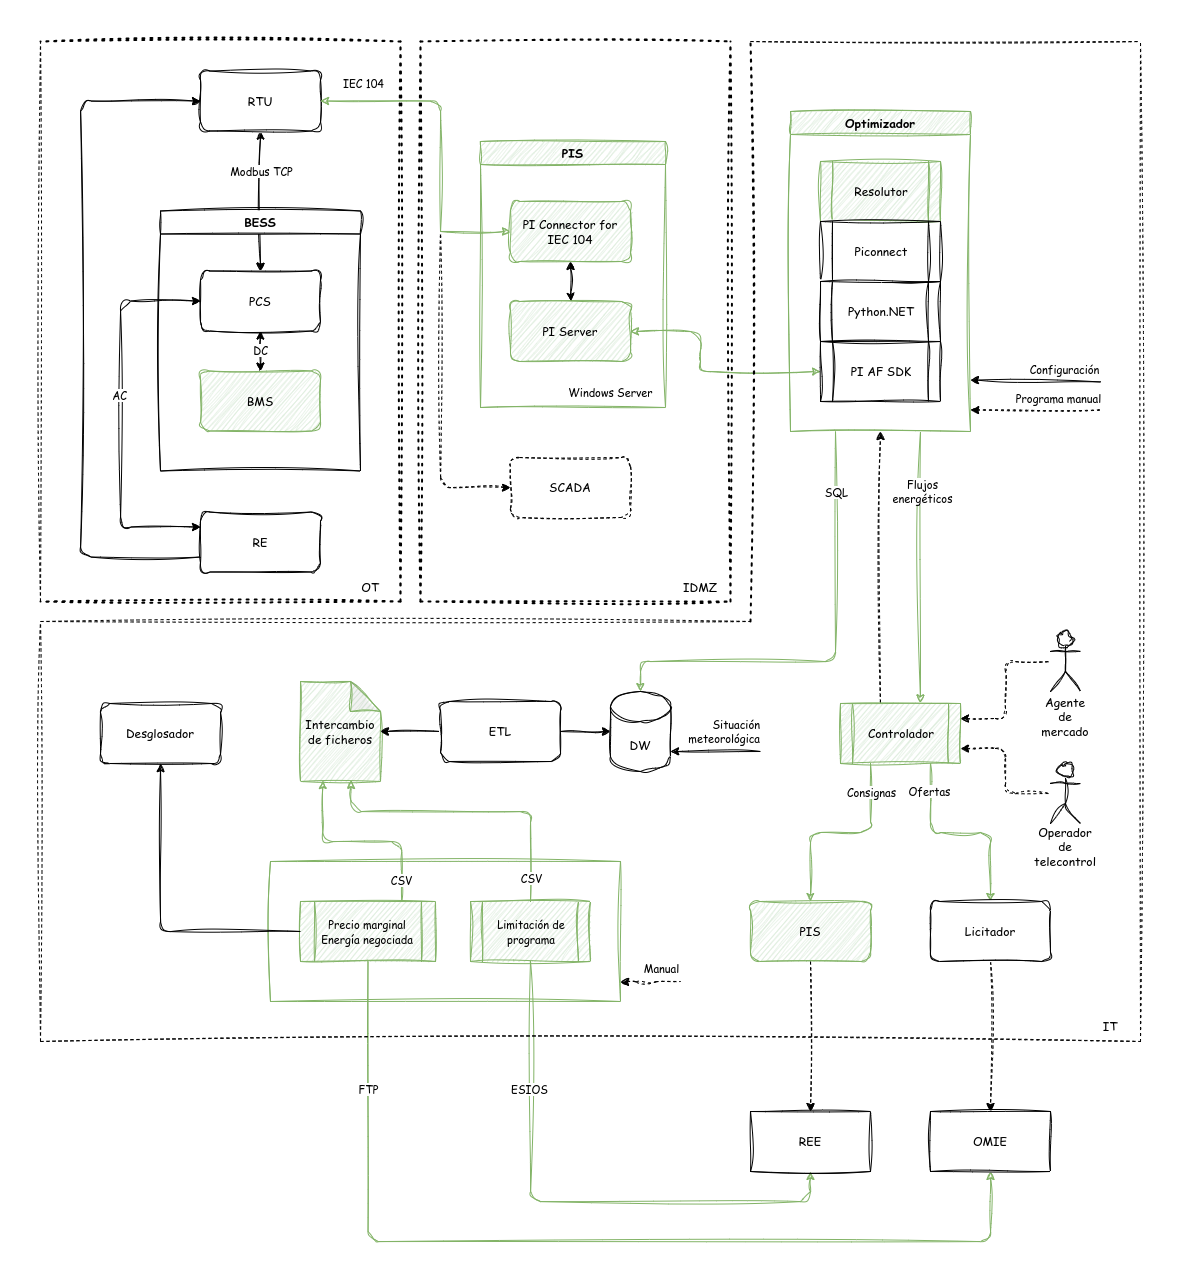
\includegraphics[width=\linewidth]{figures/arquitectura.png}
  \caption[Arquitectura del sistema.]{Arquitectura del sistema.}%
  \label{fig:arquitectura}
\end{figure}

A su vez, desde la perspectiva del cumplimiento de los objetivos secundarios, se ha buscado de la maximización de la rentabilidad mediante la optimización de las posiciones del mercado, junto con la consideración del desgaste de las baterías, ciclándolas de forma estable y controlada a través de la lógica de negocio de la modelización. Además, se han cumplido con los requisitos regulatorios, principalmente definidos por el operador del sistema en forma de límites técnicos, evitando así posibles penalizaciones económicas. Se ha garantizado la seguridad de la operación desplegando parte de la integración con la infraestructura física en una \gls{idmz}, evitando la exposición de la información de los activos energéticos a redes no autorizadas. También, el diseño mantiene una arquitectura generalizada, siendo capaz de operar en múltiples instalaciones sin modificación alguna de la lógica del sistema. Se han dado facilidades a los agentes de mercado y operadores de telecontrol para la monitorización del sistema y se ha tenido en cuenta la respuesta automática ante fallos, como la falta de disponibilidad. Finalmente, se ha efectuado un análisis de viabilidad económica donde se muestran resultados medibles.

Por otro lado, según el punto de vista de la arquitectura, después de analizar las configuraciones topológicas con las que trabaja el sistema, se ha unificado e implantado la nueva infraestructura operacional para tanto la adquisición de datos de los \glspl{bess} como el control de la carga y descarga de la misma, con el resto de componentes ya existentes de la red. Concretamente, se ha hecho uso de protocolos de comunicación industriales para intercambiar información con los activos energéticos e introducir la integración de las baterías con el \gls{pis}, que realiza la labor de historiador guardando los estados de las señales físicas a lo largo del tiempo para su posterior consulta. Con ello, se ha configurado la política de obtención de datos mediante mecanismos espontáneos y de \gls{gi} y se ha facilitado su lectura. De esta forma, se dibuja una paralela con las conocidas fases de un proyecto de \gls{iiot}, sensorización, procesamiento, gestión y actuación.

Junto a esto, se ha obtenido la información del entorno de mercado a través de las interfaces proporcionadas por las instituciones oficiales correspondientes, el \gls{mo} y el \gls{tso}. La información se ha procesado y transformado en el formato adecuado para su almacenamiento masivo en el \gls{dw}, la cual ha tenido que ser consultada eficientemente. Para ello, se ha hecho uso de procesos periódicos temporizados según los programas de mercado.

Más allá, se ha realizado un trabajo de modelización estructural de la situación física de las instalaciones, con el propósito de determinar la solución optima al problema de ciclado de energía de las instalaciones. Mediante un lenguaje de modelado abstracto, se han definido los comportamientos físicos de todos los tipos de instalaciones, desde las menos complejas, como las aisladas, a las más complejas, como las híbridas. Precisamente, se ha incorporado en el modela la lógica de la totalidad de los activos energéticos, tanto de almacenamiento como de generación.

Por último, se ha definido apropiadamente el comando y control del sistema, en forma de consignas de selección del perfil de potencia de las baterías y la vuelta al mínimo técnico de las mismas, junto con el calculo de los precios de oferta de mercado de las posiciones de compra y venta, mediante un algoritmo de oferta por semiciclo de carga. Además, para facilitar la supervisión a los agentes de mercado y operadores de telecontrol, se ha desarrollado un cuadro de mando a través del cual monitorizar el comportamiento automático del sistema y tomar el control manual si es necesario.

De esta forma, se ha habilitado el arbitraje de energía en el mercado en las instalaciones controladas. De no ser por el sistema desarrollado, al no existir ninguna otra solución alternativa desplegada en la península en la actualidad, las instalaciones a controlar registradas en el mercado tendrían que perder las oportunidades de arbitraje correspondientes o ser comandadas manualmente por los operarios de telecontrol, situación absolutamente inadmisible debido a la complejidad de la operación.

Cabe destacar que tanto los \glspl{bess} como, por lo tanto, los sistemas de optimización de baterías en el mercado eléctrico, se encuentran todavía en su infancia, por lo menos en el territorio europeo. Precisamente, según un estudio sobre el uso de las tecnologías de almacenamiento~\cite{hu2022potential}, ``el principal sistema de almacenamiento de energía en Europa sigue siendo el bombeo hidroeléctrico''. Esto significa que, viendo como el panorama de las tecnologías eléctricas pone su foco cada vez más en estas tecnologías de almacenamiento, es probable que salgan al mercado sistemas más sofisticados de control. Aunque, actualmente, las instalaciones con \glspl{bess} sean pocas en comparación al resto, las entidades energéticas buscan implantarlas en toda las instalaciones de generación para mejorar el aprovechamiento de la energía. Por ello, si bien el sistema implantado ha sido satisfactoriamente desplegado a lo largo de todo el país, quizás sea necesario tomar nuevas consideraciones al respecto y tener en cuenta dichas alternativas cuando la energía ciclada diariamente iguale o supere las cantidades de las de otros activos energéticos ampliamente asentados.

\section{Trabajo futuro}%
\label{makereference8.2}

En cuanto al trabajo futuro, \textsc{Optibat} se encuentra limitado al arbitraje en los mercados spot: diario, intradiarios y continuo. Aún así, existen otros mercados más o menos rentables~\cite{cnmc2024balance}, como los mercados de \gls{mfrr} y \gls{afrr} que negocian disponibilidades. Resulta interesante añadir soporte a estos mercados para completar así el perfil de arbitraje de estas tecnologías de almacenamiento, ya que las baterías también son idóneas para la operación en dichos mercados debido a sus altas capacidades de conmutación.

Si bien la integración con los mercados de regulación es definitivamente la mejora más notable a realizar, también aporta beneficio refinar la modelización del desgaste de las baterías~\cite{shamarova2022review}. Mediante la incorporación de señales aún más granulares y las especificaciones del \gls{bms} (adaptando el sistema a cada batería), es posible modelizar incluso el imperceptible desgaste mismo del \gls{soc} de las baterías en reposo. Ciertamente, aunque no sea un aspecto sumamente prioritario, debido al constante ciclado de las baterías que, por naturaleza, no busca precisamente el mantenimiento en estado estacionario, el aporte sustancial toma forma del aumento de fidelidad de los procesos físicos modelados. Además, un análisis en profundidad del desgaste sufrido por la batería, más allá del consumo de los ciclos para los que está calificada por el fabricante, brinda claridad a posibles optimizaciones del beneficio obtenido bajo condiciones más adversas que las experimentadas.

Junto a ello, el trabajo futuro más realista viene dado en forma de la implantación del sistema de optimización desarrollado en el creciente número de nuevas instalaciones híbridas con activos energéticos de almacenamiento en incorporación continua a la red. Como ya se ha detallado anteriormente, los \glspl{bess}, al ser todavía una tecnología no tan ampliamente establecida, se encuentran en continuo crecimiento. De hecho, incluso durante el proceso de desarrollo se hizo disponible un nuevo sistema de almacenamiento.

Cabe destacar que se han esfuerzos para el mantenimiento y mejora del trabajo desarrollado dentro de la entidad energética pertinente, con el objetivo de garantizar la continuación de su ciclo de vida, de tal forma que su operación y despliegue prosigan bajo la supervisión de un equipo diferente.
